% --
%
% Configuração do Documento
%
% --
\documentclass[10pt,brazil]{beamer}
\uselanguage{Portuguese}
\languagepath{Portuguese}
\usepackage[utf8]{inputenc}


% ---
% Pacotes adicionais
% ---
\usepackage[light,math]{kurier}         %Altera Fonte Utilizada no arquivo
\usepackage{amsmath,amsfonts,amsthm,amssymb,mathrsfs}
\allowdisplaybreaks[1]
\usepackage{microtype}
\usepackage{mathtools}
\usepackage{csquotes}
\usepackage{tikz}
\usetikzlibrary{matrix}
\usetikzlibrary{patterns}
\usepackage{faktor}
\usepackage[Sonny]{fncychap}

\usepackage{tikz}
\graphicspath{{images/}}
\usepackage[light,math]{kurier}
\usetheme{Madrid}
\useinnertheme{rectangles}


\renewcommand{\raggedright}{\leftskip=0pt \rightskip=0pt plus 0cm} %texto justificado

\usepackage[%
    alf,
    abnt-emphasize=bf,
    bibjustif,
    recuo=0cm,
    abnt-doi=expand,            % Expande um endereço iniciado com doi: para http://dx.doi.org/
    abnt-url-package=url,       % Utiliza o pacote url
    abnt-refinfo=yes,           % Utiliza o estilo bibliográfico abnt-refinfo
    abnt-etal-cite=3,
    abnt-etal-list=3,
    abnt-thesis-year=final
]{abntex2cite}   

\setbeamertemplate{theorems}[numbered] % to number
\setbeamercovered{transparent}

\theoremstyle{definition}
\newtheorem{dfn}{Definição}
\newtheorem{obs}{Observação}
\newtheorem*{proofthm}{Demonstração do Teorema}
\newtheorem*{proofprop}{Demonstração da Proposição}
\newtheorem{ex}{Exemplo}
\newtheorem{prop}{Propriedade}
\newtheorem{proposition}{Proposição}


\newcommand{\der}{\text{d}}					%Comando para fazer o d da derivada fora do ambienta matemático
\newcommand{\mb}[2]{\mathbb{#1}^{#2}}		%Comando para usar \mathbb de maneira  mais eficiente
\newcommand{\mca}[2]{\mathcal{#1}_{#2}}
\newcommand{\mul}[2]{\mu_{#1}\left(#2\right)}			%Comando para escrever a multiplicidade de modo mais eficiente
\newcommand{\mc}[2]{\mathcal{I}_{#1}\left(#2\right)}   %Comando para escrever o IPH de maneira  mais eficiente

% --
% Define Cores Personalizadas 
% --
\definecolor{ver}{RGB}{124,26,29}
\definecolor{yel}{RGB}{158,134,35}
\definecolor{ros}{RGB}{255,51,102}
\definecolor{ver1}{RGB}{169,88,99}
\definecolor{ver2}{RGB}{156,63,75}
\definecolor{ver3}{RGB}{145,43,56}
\definecolor{azul}{RGB}{18,35,97}

% --
% Customiza o título 
% --
\setbeamercolor{title}{fg=azul, bg=white!95!black}

% --
% Remove os controles de navegação 
% --
\setbeamertemplate{navigation symbols}{}

% --
% Customiza o background
% --
\setbeamertemplate{background}{
	\begin{tikzpicture}[remember picture,overlay]
	% --- LinhaInferior
	\draw[line width=0.4mm,azul] ([shift={(2.5cm,0.4cm)}]current page.south west) -- ([shift={(-0.38cm,0.4cm)}]current page.south east);
	\draw[line width=0.4mm,azul] ([shift={(-0.3cm,0.4cm)}]current page.south east) -- ([shift={(-0.26cm,0.4cm)}]current page.south east);
	\draw[line width=0.4mm,azul] ([shift={(2.75cm,0.3cm)}]current page.south west) -- ([shift={(-0.38cm,0.3cm)}]current page.south east);
	\draw[line width=0.4mm,azul] ([shift={(-0.3cm,0.3cm)}]current page.south east) -- ([shift={(-0.26cm,0.3cm)}]current page.south east);
	\draw[line width=0.4mm,azul] ([shift={(3cm,0.2cm)}]current page.south west) -- ([shift={(-0.38cm,0.2cm)}]current page.south east);
	\draw[line width=0.4mm,ver1] ([shift={(-0.3cm,0.2cm)}]current page.south east) -- ([shift={(-0.26cm,0.2cm)}]current page.south east);
	
	% --- Logo 
	\node[xshift=1.5cm,yshift=-1cm] at (current page.north west) {
\includegraphics[scale=0.15]{logo_ufmg.jpg}};
	
	\end{tikzpicture}
}

% --
% Customiza o título do frame 
% --
\setbeamercolor{frametitle}{fg=azul, bg=white} 
\makeatletter
\setbeamertemplate{frametitle}
{
	\ifbeamercolorempty[bg]{frametitle}{}{\nointerlineskip}%
	\@tempdima=\textwidth%
	\advance\@tempdima by\beamer@leftmargin%
	\advance\@tempdima by\beamer@rightmargin%
	\pgfsetfillopacity{.1}       %<------ fix filling opacity
	\begin{beamercolorbox}[sep=0.3cm,left,wd=\the\@tempdima]{frametitle}
		\usebeamerfont{frametitle}%
		\vbox{}\vskip1ex \hskip6ex%
		\if@tempswa\else\csname beamer@fteleft\endcsname\fi%
		\strut\pgfsetfillopacity{1}\insertframetitle\strut\par%  <---- text opacity
		{%
			\ifx\insertframesubtitle\@empty%
			\else%
			{\usebeamerfont{framesubtitle}\usebeamercolor[fg]{framesubtitle}\insertframesubtitle\strut\par}%
			\fi
		}%
		\vskip-1ex%
		\if@tempswa\else\vskip-.3cm\fi% set inside beamercolorbox... evil here...
	\end{beamercolorbox}%
}
\makeatother


% --
% Customimza o ambiente de Teorema 
% --
\setbeamercolor{block title}{use=structure, fg=white, bg=azul}
\setbeamercolor{block body}{use=structure, fg=black, bg=white!96!black}
\setbeamertemplate{block begin}[default]
\setbeamertemplate{block end}[default]



% --
% Customiza o footline 
% --
\setbeamertemplate{footline}{}


% --
% Customiza o headline 
% --
\setbeamertemplate{headline}
{
	\leavevmode%
	\hbox{%
		\begin{beamercolorbox}[wd=\paperwidth,ht=9.25ex,dp=3.5ex]{ver}%
			\raggedright
			\hspace*{2em}%
			\hspace*{2em}%
		\end{beamercolorbox}%
	}%
}


% --
% Customiza o estilo dos ambientes Itemize e Enumerate 
% --
\setbeamertemplate{enumerate item}{\color{azul}\insertenumlabel)}
\setbeamertemplate{enumerate subitem}{\color{azul}\insertenumlabel.\insertsubenumlabel)}
\setbeamertemplate{enumerate subsubitem}{\color{azul}\insertenumlabel.\insertsubenumlabel.\insertsubsubenumlabel)}
\setbeamertemplate{enumerate mini template}{\insertenumlabel}

\setbeamertemplate{itemize item}{\scriptsize\raise1.25pt\hbox{\color{azul}\donotcoloroutermaths$\bullet$}}
\setbeamertemplate{itemize subitem}{\tiny\raise1.5pt\hbox{\color{azul}\donotcoloroutermaths$\blacksquare$}}
\setbeamertemplate{itemize subsubitem}{\tiny\raise1.5pt\hbox{\color{azul}\donotcoloroutermaths$\blacktriangleright$}}

% -- 
% Customiza o estilo do Table of Contents 
% --
\setbeamertemplate{section in toc}[square]

\setbeamerfont{section number projected}{size=\large}
\setbeamercolor{section number projected}{bg=white!95!black, fg=azul}

\setbeamertemplate{subsection in toc}{%
	\leavevmode\leftskip=5.65ex%
	\llap{\raisebox{0.2ex}{\textcolor{azul}{$\blacktriangleright$}}\kern1ex}%
	\inserttocsubsection\par%
}

% -- 
%Customiza as margens dos frames 
% -- 
\setbeamersize{text margin left=1cm,text margin right=1cm}

% -- 
% Apresentação
% -- 
\begin{document}
\mode<presentation>

% -- 
% Info
% -- 
\title[]{ANÁLISE DE DADOS UTILIZANDO CLUSTER DE BAIXO CUSTO}
\subtitle{COMPARAÇÃO DE DESEMPENHO DE AMBIENTES VIRTUAIS}

\institute[UFMG]{Universidade Federal de Minas Gerais}

\author[Felipe Rocha]{Felipe Fonseca Rocha \\
  \vspace{0.25cm}
  Orientador: Ítalo Fernando Scotá Cunha }
\date{09 de Fevereiro de 2022}

% --
% Inclui o sumário antes de cada seção
% --
\AtBeginSection{%
  \begin{frame}
    \tableofcontents[currentsection, subsectionstyle=show/show/hide]
  \end{frame}
}
% -- 
% Cria slide com título
% -- 
\frame{\maketitle}

% -- 
% Cria slide com sumário
% -- 

\begin{frame}{Sumário}
  \tableofcontents
\end{frame}

% 	\begin{figure}
% 		\centering
% 		\includegraphics[scale=0.45]{objetivo.jpg}
% 	\end{figure}

% --
%
% Conteúdo 
%
% --

% -- 
% Objetivos
% -- 
\section{Objetivo}

\begin{frame}{Objetivo}
  Realizar a comparação de desempenho de orquestração de recursos em cluster de baixo custo em ambientes virtualizados:
  completa,
  Sistema Operacional; para o processamento e a análise de dados em saúde, como tendência de consumo de azitromicina entre os anos 2014 e 2021.
\end{frame}

% -- 
% Objetivos - Específicos
% -- 
\subsection{Objetivos específicos}

\begin{frame}
  \begin{itemize}
    \item Realizar a orquestração de recursos em cluster de baixo custo;
    \item Comparar o desempenho de clusters em ambientes virtualizados;
    \item Validar o uso de um cluster de utilização compartilhada para processamento de dados distribuídos;
    \item Propor um método de análise em cluster Kubernetes\textregistered com uso de computadores desktops;
  \end{itemize}
\end{frame}

% -- 
% Introdução
% -- 
\section{Introdução}

% -- 
% Introdução - Motivação
% -- 
\subsection{Motivação}

\begin{frame}{Introdução - Motivação}
  \begin{itemize}[]
    \item Uso de ferramentas de analise dados em saúde \cite{galvao_desafios_2019}
    \item Integração de Sistemas de Informação em Saúde e necessidade de facilitar processo de análise de grandes volumes de dados \cite{galvao_desafios_2019,mehta_concurrence_2018}
    \item Disponibilidade de dados pelo Decreto nº 8.777 \cite{brasildisponibilidade2016} e a necessidade de extração de informações.
  \end{itemize}
\end{frame}


% -- 
% Introdução - Justificava
% -- 
\subsection{Justificativa}

\begin{frame}{Introdução - Justificativa}
  \begin{columns}
    \begin{column}{0.5\textwidth}
      \begin{itemize}
        \item Restrição Orçamentária
              \begin{itemize}
                \item Diminuição de verbas para ciência e técnologia $-2,32\%$
                \item Aumento do dólar em mais de $3,27\%$
              \end{itemize}
        \item Disponibilidade de estratégias de analise
      \end{itemize}
    \end{column}
    \begin{column}{0.5\textwidth}  %%<--- here
      \begin{center}
        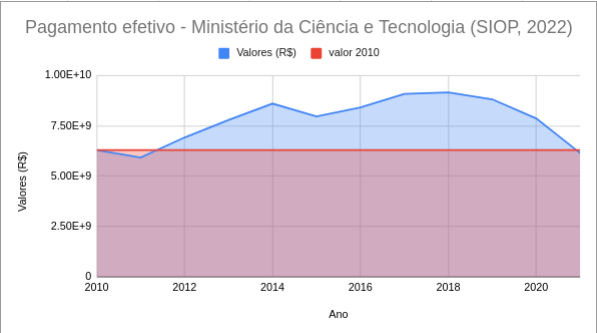
\includegraphics[width=1\textwidth]{orcamento.png}
        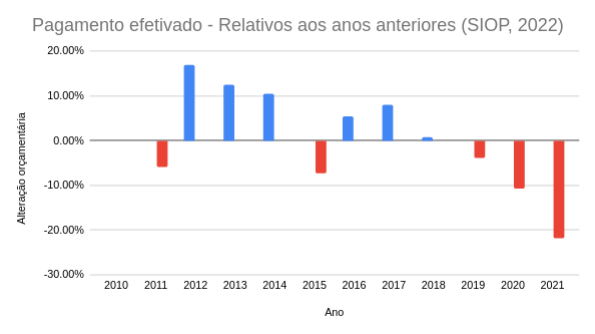
\includegraphics[width=1\textwidth]{variacaoorcamentaria.png}
      \end{center}
    \end{column}
  \end{columns}
\end{frame}

\begin{frame}{Introdução - Justificativa}
  \begin{columns}
    \begin{column}{0.5\textwidth}
      \begin{itemize}
        \item Restrição Orçamentária
              \begin{itemize}
                \item Diminuição de verbas para ciência e técnologia $-2,32\%$
                \item Aumento do dólar em mais de $3,27\%$
              \end{itemize}
        \item Disponibilidade de estratégias de análise
        \item Tomada de decisão em saúde, mais de 152mi de Brasileiros dependem exclusivamente do SUS (UNASUS, 2021)
      \end{itemize}
    \end{column}
    \begin{column}{0.5\textwidth}  %%<--- here
      \begin{center}
        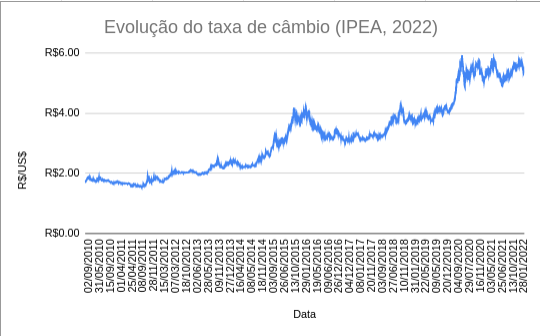
\includegraphics[width=1\textwidth]{variacaodolar.png}
      \end{center}
    \end{column}
  \end{columns}
\end{frame}

% -- 
% Introdução - Abordagem
% --
\subsection{Abordagem}
\begin{frame}{Introdução - Abordagem}
  \begin{itemize}

    \item Cluster Kubernetes\textregistered
    \item Cargas de trabalho - Analise de tendencia de uso de azitromicina entre 2014 e 2021
    \item 2 abordagens de virtualização:
          \begin{itemize}
            \item completa - \emph{Hypervisor} tipo 2
            \item sistema operacional - contêineres
          \end{itemize}
    \item Máquinas comuns e de baixo poder computacional:
          \begin{itemize}
            \item 1 vCPU
            \item 2 GB de RAM
            \item 6-8 máquinas
          \end{itemize}
  \end{itemize}
\end{frame}

\begin{frame}{Introdução - Abordagem}
  \begin{itemize}
    \item Aplicação de abordagem DevOps:
          \begin{itemize}
            \item \emph{Shift Right} - Fazes finais do \emph{SDLC}
            \item CI (integração contínua) e CD (entrega contínua) - deploy da aplicação e inicio do monitoramento
            \item IaC (infraestrutura como código) - acuracia na repetição dos procedimentos de provisionamento de recursos e configuração.
          \end{itemize}
    \item Uso de metodos do tipo USE (utilização, saturação e erro) para comparação entre as cargas de trabalhos e ambientes de simulação e virtualização
  \end{itemize}
\end{frame}


% -- 
% Revisão de Literatura
% -- 
\section{Revisão de literatura}

% -- 
% Revisão de Literatura - Análise de dados
% -- 
\subsection{Análise de dados}

\begin{frame}{Revisão de literatura- Análise de dados}
  \begin{itemize}
    \item Complexidade de tomar descisão em saúde \cite{andrade_tomada_2008,resende2009}
    \item Definição de Big Data 5 Vs, complexidade e Destruturação  \cite{laney20013d,oracle2013,intel2012}
    \item Complexidade de relacionar dados por multifatoriedade \cite{faceli2011}
    \item Não consolidação de métodos de uso de Big Data em saúde, especialmente em estudos quantitativos, foco em custo e decisões clínicas \cite{nishita2018}
  \end{itemize}
\end{frame}

% -- 
% Revisão de Literatura - Alternativas open source
% -- 
\subsection{Alternativas open source}

\begin{frame}{Revisão de literatura- Alternativas open source}
  \begin{itemize}
    \item Agrupamento em categorias:
          \begin{itemize}
            \item Computação em nuvem privada:
                  \begin{itemize}
                    \item Tecnologias: OpenStack\textregistered, CloudStack\textregistered

                    \item Requisitos exigentes
                    \item Complexidade: SaaS, PaaS e SaaS \cite{openstack,cloudstack,mell_nist_2011}
                  \end{itemize}

          \end{itemize}
  \end{itemize}
\end{frame}


\begin{frame}{Revisão de literatura- Alternativas open source}
  \begin{columns}
    \begin{column}{0.5\textwidth}
      \begin{itemize}
        \item Orquestração de Containers:
              \begin{itemize}
                \item Kubernetes\textregistered
                \item Apache Mesos\textregistered
                \item Hashicorp Nomad\textregistered
                \item Docker Swarm\textregistered
              \end{itemize}
      \end{itemize}
    \end{column}
    \begin{column}{0.5\textwidth}  %%<--- here
      \begin{center}
        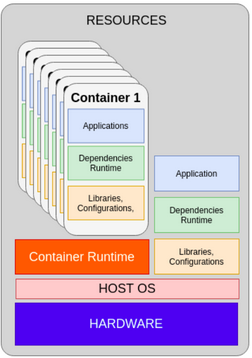
\includegraphics[width=0.5\textwidth]{containers.png}
        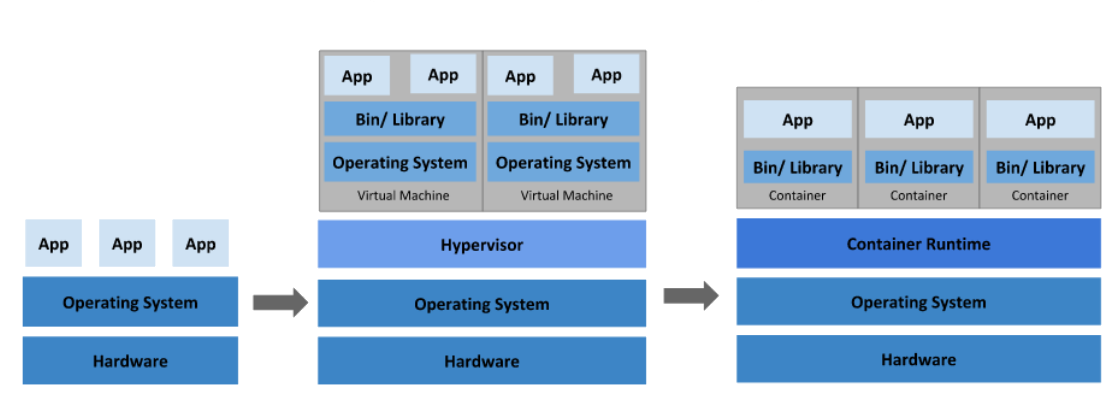
\includegraphics[width=1\textwidth]{vmsContainer.png}
      \end{center}
    \end{column}
  \end{columns}
\end{frame}

% -- 
% Revisão de Literatura - Cluster orquestrador de container
% -- 
\subsection{Cluster orquestrador de container}

\begin{frame}{Revisão de literatura- Cluster orquestrador de container}
  \begin{columns}
    \begin{column}{0.5\textwidth}
      \begin{itemize}
        \item Kubernetes\textregistered:
              \begin{itemize}
                \item Origem de 15 anos de trabalho da Google (Borg) \cite{verma_large-scale_2015}
                \item estrutura de objetos componentizados \cite{kubernetes2022}
                      \begin{itemize}
                        \item Kube-apiserver
                        \item Kube-scheduler
                        \item Kube-controller-manager
                        \item Kubelet
                        \item Kube-proxy
                        \item Pod
                      \end{itemize}
              \end{itemize}
      \end{itemize}
    \end{column}
    \begin{column}{0.5\textwidth}  %%<--- here
      \begin{center}
        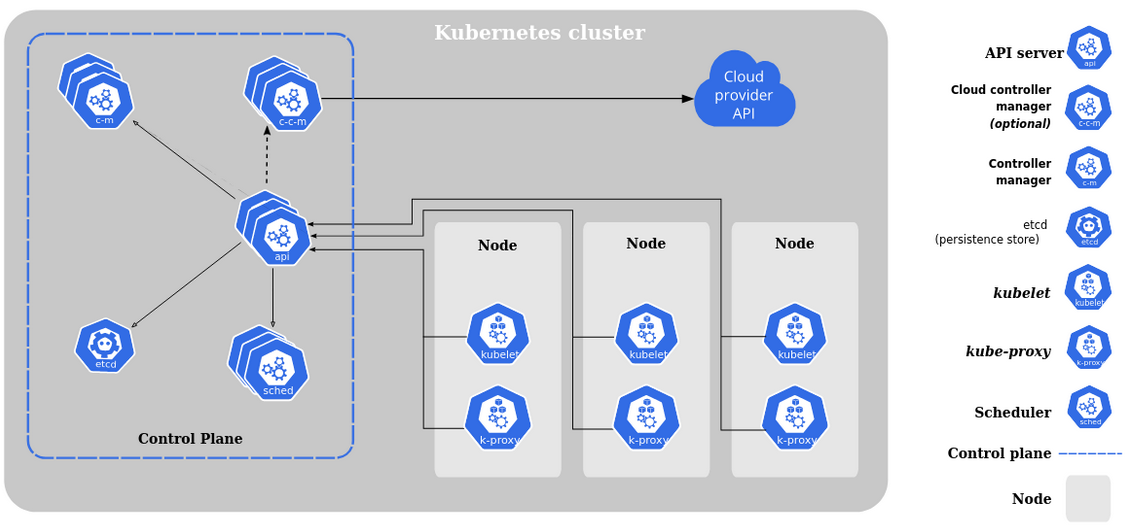
\includegraphics[width=1\textwidth]{kubeadm-node.png}
      \end{center}
    \end{column}
  \end{columns}
\end{frame}

% -- 
% Métodos
% -- 
\section{Método}

% -- 
% Método - Disponibilidade dos recursos deste trabalho
% -- 
\subsection{Disponibilidade dos recursos deste trabalho}

\begin{frame}{Método - Disponibilidade dos recursos deste trabalho}
  Todos os componentes definidos nesse trabalho estarão contidos em um ou mais repositórios públicos, garantindo assim a livre apreciação da comunidade não só científica, mas a todos os interessados na contribuição ou utilização sob a licença pública geral GNU versão 3 \cite{foss2022}.
  \hyperlinkpresentationend{https://github.com/felipefrocha/esufmg-tcc Repositório}
\end{frame}

% -- 
% Método - Especificação dos nós integrantes cluster de baixo custo
% -- 
\subsection{Especificação dos nós integrantes cluster de baixo custo}

\begin{frame}{Método - Especificação dos nós integrantes cluster de baixo custo}
  \begin{columns}
    \begin{column}{0.5\textwidth}
      \begin{itemize}
        \item Cluster Simulado:
              \begin{itemize}
                \item Virtualização:
                      \begin{itemize}
                        \item Maquinas Virtuais (VMs) (\emph{Hypervisor} tipo 2)
                        \item Contêineres Aninhados (Docker In Docker, ou DinD)
                      \end{itemize}
                \item Especificações de hardware 1vCPU, 2 GB de RAM;
              \end{itemize}
        \item provisionamento em 2 etapas
        \item máquinas subutilizadas
        \item CAPEX

      \end{itemize}
    \end{column}
    \begin{column}{0.5\textwidth}  %%<--- here
      \begin{center}
        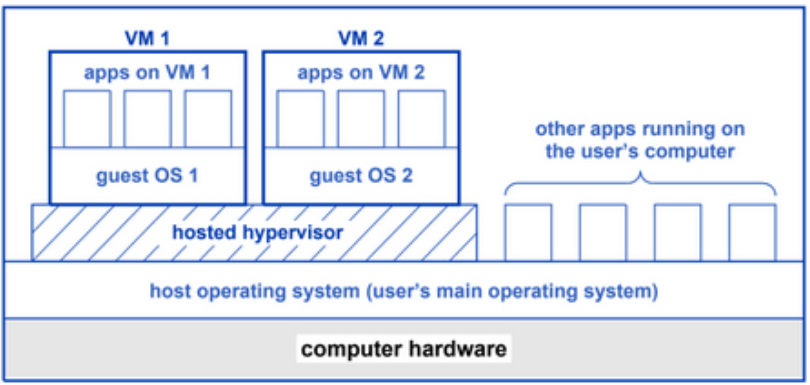
\includegraphics[width=1\textwidth]{vms.png}
      \end{center}
    \end{column}
  \end{columns}
\end{frame}


% -- 
% Método - Plataforma de orquestração de carga de trabalho
% -- 
\subsection{Plataforma de orquestração de carga de trabalho}

\begin{frame}{Método - Plataforma de orquestração de carga de trabalho}
  \begin{columns}
    \begin{column}{0.5\textwidth}
      \begin{itemize}
        \item Multi-master Etcd atachado \cite{kubernetes2022, etcd2022}
        \item Arquitetura sugerida para produção
        \item Alta disponibilidade do cluster
        \item Recursos limitados
      \end{itemize}
    \end{column}
    \begin{column}{0.5\textwidth}  %%<--- here
      \begin{center}
        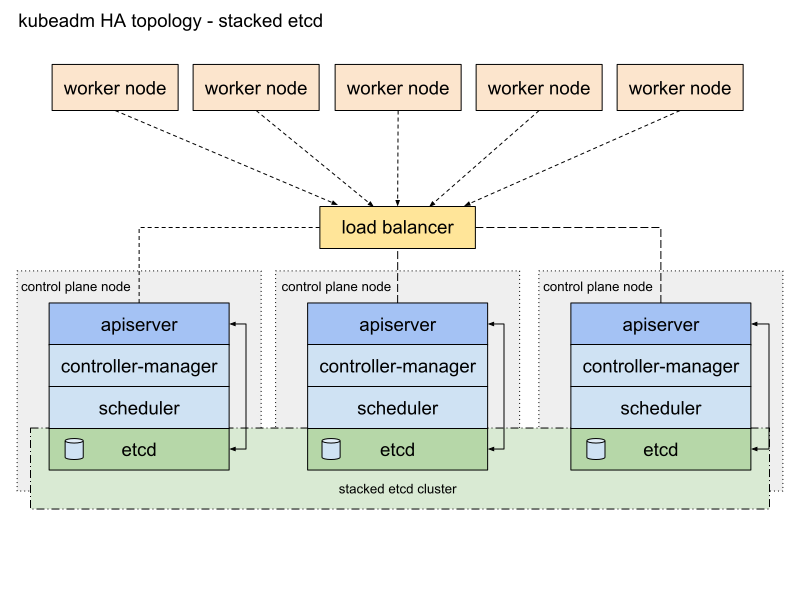
\includegraphics[width=1\textwidth]{kubeadm-ha-topology-stacked-etcd.png}
      \end{center}
    \end{column}
  \end{columns}
\end{frame}

\begin{frame}{Método - Plataforma de orquestração de carga de trabalho}
  \begin{itemize}
    \item Implantação da carga de Trabalho
          \begin{itemize}
            \item Container
            \item Parametrizável
            \item Volume compartilhado
          \end{itemize}
    \item Ciclo de vida da aplicação
          \begin{itemize}
            \item Monorepo \cite{brito_monorepos_2018}
            \item Padronização de código
            \item Sincronização
            \item Deploy em Pipeline
          \end{itemize}
  \end{itemize}
\end{frame}

% -- 
% Método - Configuração e provisionamento do cluster
% -- 
\subsection{Configuração e provisionamento do cluster}

\begin{frame}{Método - Configuração e provisionamento do cluster}
  \begin{itemize}
    \item Gerenciador de Congiração (Ansible\textregistered)
    \item \emph{Agentless}
    \item Idempotência
    \item Gerenciamento de inventário
    \item SSH - Escolha do algoritimo de criptografia \cite{noauthor_rfc4254_nodate}
  \end{itemize}
\end{frame}

% -- 
% Método - Análise de dados
% -- 
\subsection{Análise de dados}

\begin{frame}{Método - Análise de dados}
  \begin{itemize}
    \item “Vendas de Medicamentos Controlados e Antimicrobianos - Medicamentos Industrializados”
    \item $530 \cdot 10^{6}$ linhas com mais de 70 GB
    \item Análise de tendência do consumo de azitromicina
    \item Caso base - comparação com processo de análise em \emph{bare metal} 8vCPU, 16 GB de RAM - totalizando o poder computacional total do cluster proposto
  \end{itemize}
\end{frame}

% -- 
% Método - Monitoramento
% -- 
\subsection{Monitoramento}

\begin{frame}{Método - Monitoramento}
  \begin{itemize}
    \item \emph{OpenTelemetry}
    \item \emph{Prometheus} Monitoramento de sistemas e Banco de dados de series temporais
    \item \emph{Grafana} - Dashboard e observabilidade
    \item Parametros de tempo, taxa de utilização de memoria e processamento
  \end{itemize}
\end{frame}


% -- 
% Método - Comparação entre tipos de virtualização
% -- 
\subsection{Comparação entre tipos de virtualização}

\begin{frame}{Método - Comparação entre tipos de virtualização}
  \begin{itemize}
    \item A arquitetura x86 comum e maior poder computacional \cite{fayyad_benchmarking_2013}
    \item macrobenchmark (system level benchmark) \cite{huge2008,scheepers2014virtualization}
    \item Parametros de tempo, taxa de utilização de memoria e processamento
    \item Maquina hospedeira e virtuais serão avaliadas durante o processamento
    \item Metodo USE de avaliação \cite{greg2022}
    \item APM Application Performance Management) associada a aplicação da carga de trabalho por \emph{OpenTelemetry} \cite{tang2021systematical}
  \end{itemize}
\end{frame}


% -- 
% Método - Cronograma
% -- 
\subsection{Cronograma}

\begin{frame}[plain]
  \hspace*{-10mm}
  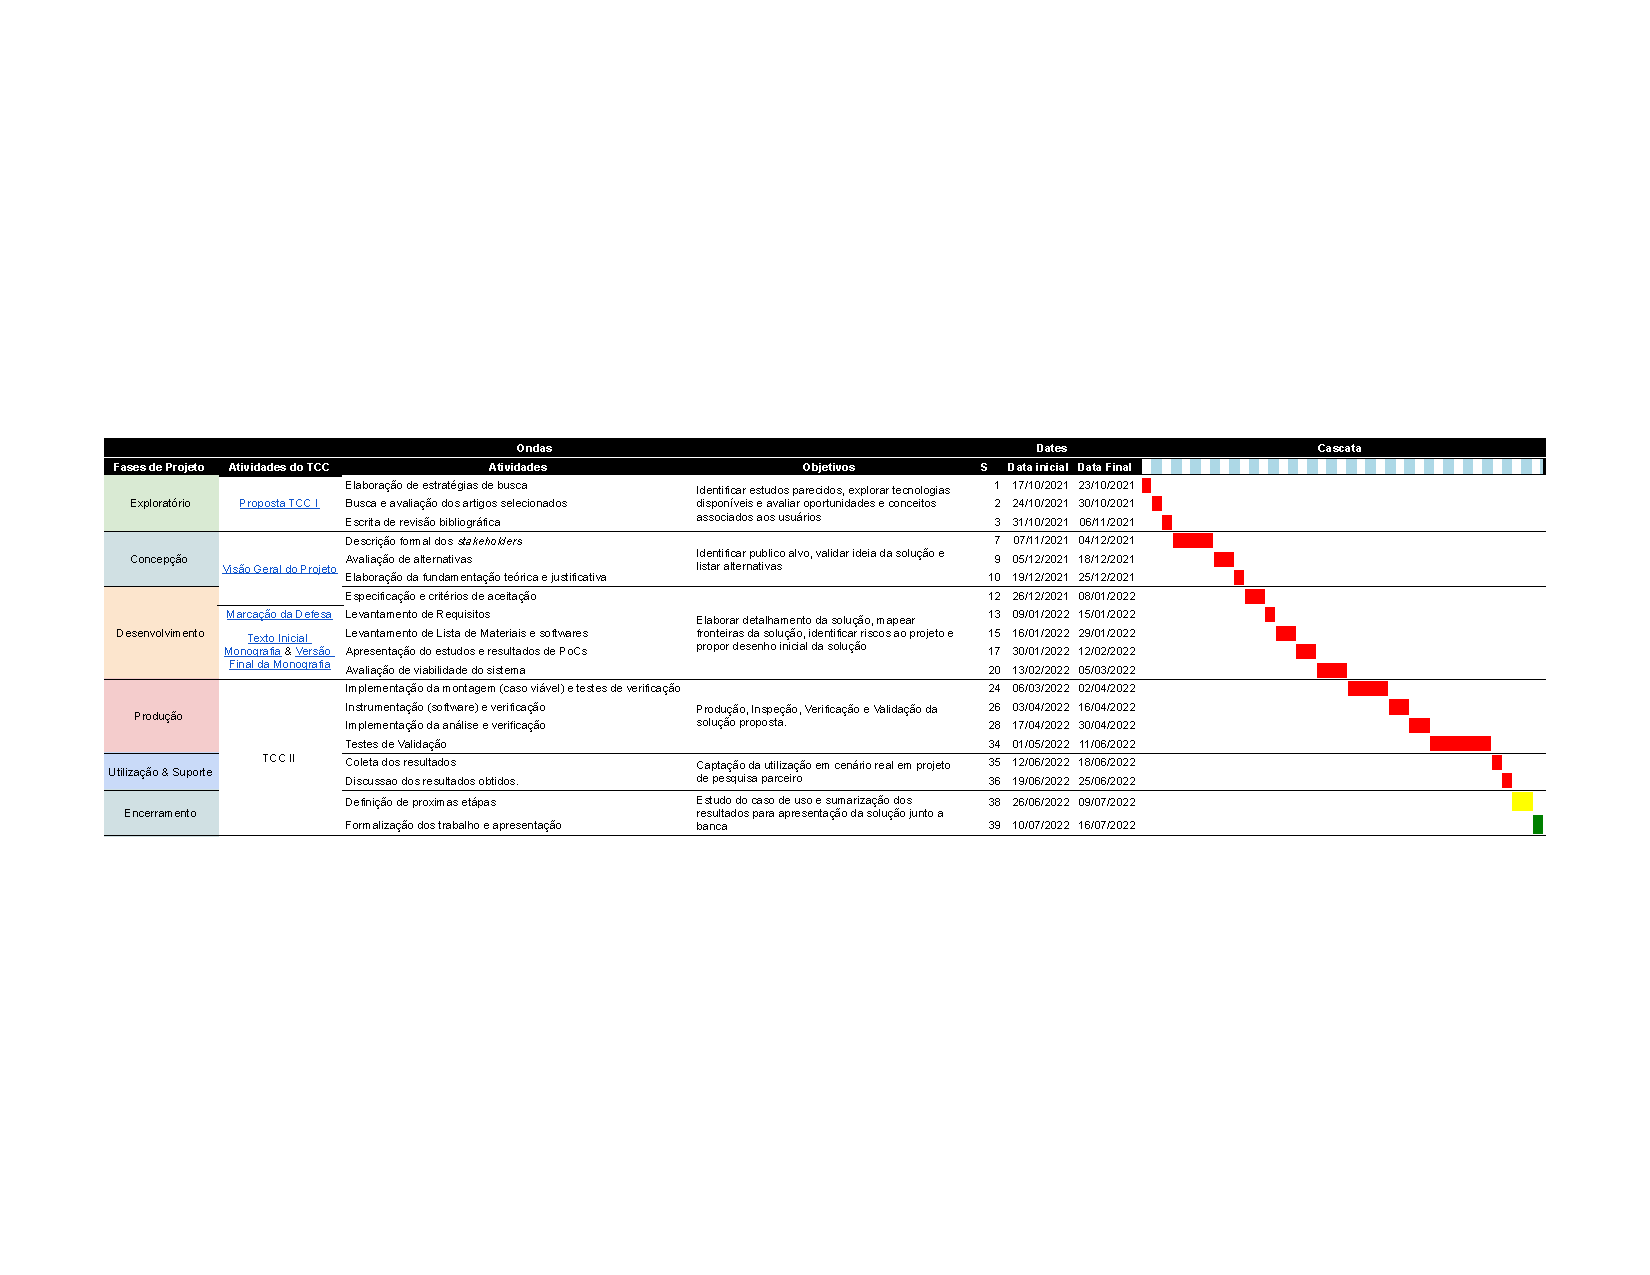
\includegraphics[width=\paperwidth]{TCC cronograma - Sheet1.pdf}
\end{frame} 

% -- 
% Conclusão
% -- 
\section{Conclusão}

\begin{frame}{Conclusão}
  \begin{itemize}
    \item Avaliação de diferentes tipos de virtualização
    \item Seleção de plataforma de orquestração de cargas de trabalhos com base em requisitos e restrições
    \item Analise dos impactos socio-econômicos oriundos da restrição orçamentária a pesquisa de uma forma geral
    \item Desenho de uma estratégia de extração de informações relevantes de uma base de dados com volume considerável
    \item Entendimento da complexidade dos fatores considerados no processo de descisão em saúde
  \end{itemize}
  Trabalhos futuros contemplarão a implementação, testes e coletas de dados para avaliação comparativa das virtualizações propostas no ambiente simulado. Baseado nesses resultados pode se evoluir essa discussão na forma de recrutamento de computadores para o cluster de maneira a garantir o isolamento da maquina base.
\end{frame} 

% -- 
% Referências
% -- 
\begin{frame}[allowframebreaks]{Referências}
  \small
  %	\nocite{*}
  %    \bibliographystyle{apalike}
  \bibliography{Apresentacao}
\end{frame}


\begin{frame}
  \centering
  {\color{ros} OBRIGADO\\
    :)}
\end{frame}
\end{document}